\documentclass{llncs}
\usepackage[utf8]{inputenc}
\usepackage{booktabs}
\usepackage{rotating}
\RequirePackage{graphicx}
\RequirePackage[spanish]{babel}
\RequirePackage[utf8]{inputenc}
\selectlanguage{spanish}
\usepackage{verbatim} 


\newcommand{\mykeywords}[1]{\par\addvspace\baselineskip \noindent \textbf{Palabras Claves:} \enspace\ignorespaces#1}

\newtheorem{teo}{Teorema}

\begin{document}

\title{Declarative Programming Report.\\ Sudoku Hidato}

\author{
  Dayrene Fundora \email{dayfundoraglez@gmail.com}\institute{Faculty of Mathematics and Computation (MATCOM), \\University of Havana (UH), Cuba.}
  }

\titlerunning{Declarative Programming Report} 
\authorrunning{Dayrene Fundora}


\maketitle

\section{Preliminaries. Randomness}
Randomness was achieved through the \texttt{System.Random}\cite{baeza} module and the main functions used were \texttt{random} to obtain an arbitrary value, \texttt{randomR} to generate random numbers in a range, and \texttt{randoms} to construct an infinite sequence of random values. Such an infinite sequence is used by almost all the functions of the implementation from indexes that indicate which value is to be used and it has been essential since \texttt{random} and \texttt{randomR} ~(Figura\ref{rand}) both receive a \texttt{RandomGen} type object~(a \emph{random} generator) which can be built manually with the \texttt{mkStdGen} function from a ``seed''  value where, due to Haskell's referential transparency, it must vary so that \texttt{mkStdGen} and therefore, random and randomR return different values in each call.


%que puede construirse manualmente con la funci\'on \texttt{mkStdGen} cuya signatura es \texttt{mkStdGen :: Int -> StdGen}
\section{Representation}
The Hidatos have been represented as a triple $(M, I, F)$ where $I$ is the position where the minimum value of the board is located, $F$ the position of the maximum value and $M$ a matrix of $n$ rows and $m$ columns where:
\begin{itemize}
\item the boxes that must be filled in to complete the sudoku have a value of $-2$
\item the boxes with a predefined value have an arbitrary number between $1$ and $k$, where it is said that $k$ is \emph{the size of hidato} \footnote{The value $1$ has been kept as the minimum to generate all the hidato and the maximum value coincides with its size.}
\item there are ``fictitious'' boxes that serve to simulate the shape of the Hidato and have a value of $negative 1$.
\end{itemize}

Figure \ref{hidato} shows an example of a Hidato with this representation.

\begin{figure}
\begin{center}
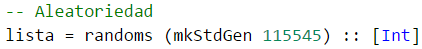
\includegraphics[width= .8\columnwidth]{figuras/lista}
\end{center}
\caption{
	``Global'' sequence of \emph{random} values in the implementation. The value \texttt{mkStdGen} receives to build it can be changed manually by any other.}
\label{listar}
\end{figure}

\begin{figure}
\begin{center}
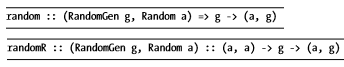
\includegraphics[width= .7\columnwidth]{figuras/rand}
\end{center}
\caption{Signature of \texttt{random} and \texttt{randomR}. Taken from \cite[p.191, p.194]{baeza}}
\label{rand}
\end{figure}

\begin{figure}
\begin{center}
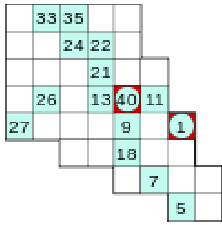
\includegraphics[width= 0.3\columnwidth]{figuras/sudoku}
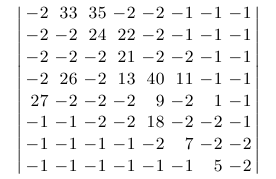
\includegraphics[width= 0.48\columnwidth]{figuras/matrep}
\end{center}
\caption{Sudoku Hidato size 40 on the left and its matrix representation on the right.}
\label{hidato}
\end{figure}





\begin{comment}
\begin{center}
$\left| 
\begin{array}{rrrrrrrr}
-2 & 33 & 35 & -2 & -2 & -1 & -1 & -1 \\
-2 & -2 & 24 & 22 & -2 & -1 & -1 & -1 \\
-2 & -2 & -2 & 21 & -2 & -2 & -1 & -1 \\
-2 & 26 & -2 & 13 & 40 & 11 & -1 & -1 \\
27 & -2 & -2 & -2 & 9 & -2 & 1 & -1 \\
-1 & -1 & -2 & -2 & 18 & -2 & -2 & -1 \\
-1 & -1 & -1 & -1 & -2 & 7 & -2 & -2 \\
-1 & -1 & -1 & -1 & -1 & -1 & 5 & -2
\end{array} 
\right|$
\end{center}
\end{comment}

\section{Generating Hidatos}
Essentially, the procedure that is carried out is to generate a solution and from it choose the boxes that will be left with preset values.

\subsection{Create a Solution}
Given that a Hidato could also be represented as a sequence of cells that describe the ``path'' formed by the sequence of numbers that begins at 1 and ends at the size of the Hidato, the solutions are constructed using a recursive idea: Given the current position that it occupies, what is the next step to take considering the 8 options \footnote{Left, right, up, down and the 4 diagonal movements~(Figure \ref{movs}).} available?
This choice is made at random each time over the set of neighboring cells:
\begin{itemize}
\item to which no value has been assigned,
\item in the case that they are outside the limits of the current matrix, the new matrix will have one more row and/or column, so the selected position is not an outside step~(Figure \ref{camino}).
\end{itemize}


\begin{figure}
\begin{center}
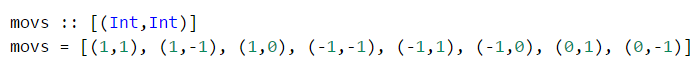
\includegraphics[width= 1\columnwidth]{figuras/movs}
\end{center}
\caption{The 8 movement options from a tile.}
\label{movs}
\end{figure}


\begin{figure}
\begin{center}
$\left| 
\begin{array}{r}
1
\end{array} 
\right|$
\end{center}

\begin{center}
$\left| 
\begin{array}{rr}
1 & 2
\end{array} 
\right|$
\end{center}

\begin{center}
$\left| 
\begin{array}{rrr}
1 & 2 & -1 \\
-1 & -1 & 3 \\
\end{array} 
\right|$
\end{center}
\caption{
	Increase of the matrix according to the steps taken. When placing $2$ on the board, the new matrix contains a column more to the right and when placing $3$, a new column appears on the right and a row more.}
\label{camino}
\end{figure}

Only one outer tile is chosen if there is no neighbor that is empty to reinforce the ``density'' of the sudoku game. We start from the matrix that has a single row and a column and it is considered a stop case when the value to be placed is the size that the Hydato is expected to have.

\subsection{Choose Default Values}
Once a solution is built, it is determined which cells will be empty and which cells will have default values. When developing the implementation, several ideas came up:

\begin{itemize}
\item Choose boxes randomly to prefix: in this case the Hidato is not guaranteed to have a unique solution.
\item Choose which values of the board will be prefixed: specifically each time a number is arbitrarily chosen, its value and the value of the successor of its successor are prefixed on the board, thus restricting the number of places that the number in the center can occupy. Although this strategy is less fast than the first~(since when determining the value to be prefixed, it requires detecting what position it occupies in the built solution) and it does not guarantee that the Hydato solution is unique, if it solves at least by reducing the amount of solutions.
\end{itemize}

These ideas are materialized with the functions \texttt{select\_no\_empty} and \texttt{select\_better\_no\_empty}~(Figure \ref{select}) respectively. 35 \% of the cells are filled, without considering those that contain the minimum and maximum value of the board, which will always be preset. It may be that increasing this percentage will guarantee the uniqueness of the solution but reduce the complexity of the ``game''.

\begin{figure}
\begin{center}
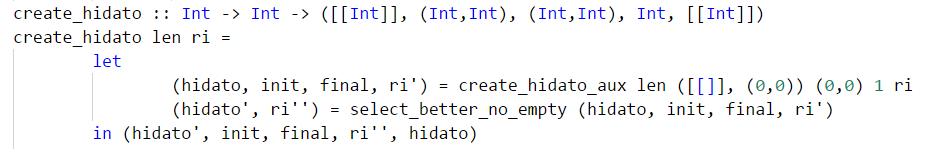
\includegraphics[width= 1\columnwidth]{figuras/createh}
\end{center}
\caption{Function by which a Hidato is created. The parameter \texttt{len} is the size of the Hidato to be built and \texttt{ri} is the index of the list of random values from which to start working.}
\label{create}
\end{figure}




\begin{figure}
\begin{center}
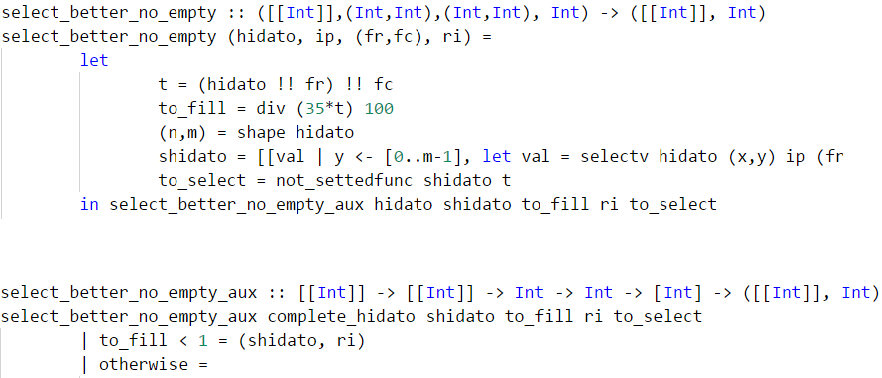
\includegraphics[width= 1\columnwidth]{figuras/select}
\end{center}
\caption{Segments of the functions by which the default values are determined.}
\label{select}
\end{figure}
\section{Solving Hidatos}
To know the number of solutions of a given Hidato, the function that detects them exploits all the possibilities exhaustively~(Figure \ref{solver}). The idea is essentially recursive and defines that, given a position on the board, the solutions of the same will be those obtained from placing the next value of the path in each of the boxes that can be placed from the actual position. We start from the position where the minimum value of the board is located and the base cases are those in which the next value of the path is the maximum number and it is in a neighboring position to your location.


Of course, the procedure can be modified so that the recursion ends when a solution is found, but it was proceeded in this way to evaluate the strategy of prefixing the Hidato values. Either way, the problem of solving a Hidato can be reduced to the Boolean Satisfaction Problem, which is considered an NP-complete problem \cite{serio}.

\section{Start the ``Game''}
Using the function \texttt{hidatos\_list} with signature \texttt{hidatos\_list :: Int -> Int -> Int -> String}~(\texttt{hidatos\_list n len ri}) it is specified that you want to generate and solve $n$ Hidatos of size $len$.
By functions defined in \texttt{Utils.hs} the Hidato and all its solutions are printed. The value $ri$ in this call must be assigned the value $0$ as shown in Figure \ref{main} to start using the sequence of random numbers from the beginning.

\begin{figure}
\begin{center}
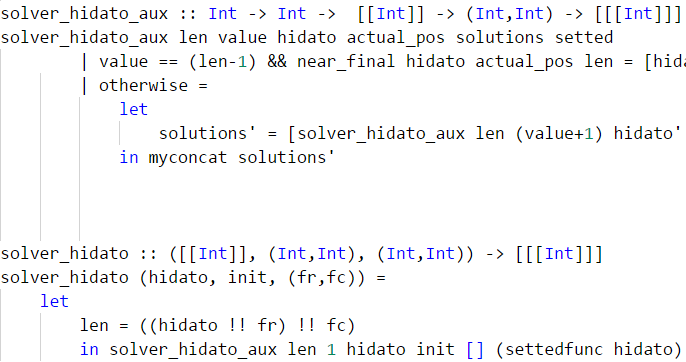
\includegraphics[width= 1\columnwidth]{figuras/solver}
\end{center}
\caption{Segments of the functions through which the Hidato is solved.}
\label{solver}
\end{figure}

\begin{figure}
\begin{center}
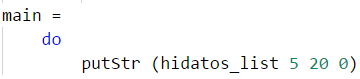
\includegraphics[width= .5\columnwidth]{figuras/main}
\end{center}
\caption{Example of invoking the ``game'' in \ texttt{Main.hs}}
\label{main}
\end{figure}


\begin{figure}
\begin{center}
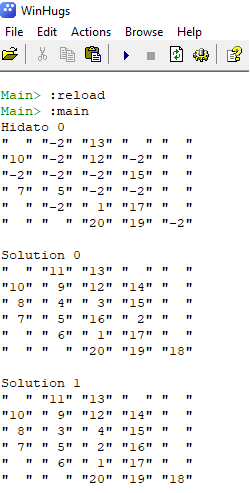
\includegraphics[width= .5\columnwidth]{figuras/corrida}
\end{center}
\caption{Section of the output of the ``Game '' with the invocation of Figure \ref{main}.}
\label{corrida}
\end{figure}
\begin{thebibliography}{5}  
\bibitem{baeza}
    Lipovaca, Miran: 
    Learn you a Haskell for a great good!,
    Cap9, Randomness,
    2011.
    
\bibitem{serio}
	Barto{\v{s}}, Samuel:
	Effective encoding of the Hidato and Numbrix puzzles to their CNF representation,
	Univerzita Karlova, Matematicko-fyzik{\'a}ln{\'\i} fakulta,
	2014
\end{thebibliography}
\end{document}